\chapter{Introduction}\label{chap:intro}

Consistency among multiple interleaved transactions in a web service context has always been an issue for researchers and database administrators. Isolation and atomicity are two of the four \gls{acid} properties that are often relaxed in order to prevent a performance bottleneck. However, when these properties are relaxed, the database can reach an inconsistent state when concurrent transactions interleave incorrectly. This causes data to become corrupted, expensive compensation transactions to be executed, and cascading rollbacks on multiple nodes to be completed before processing can continue. 

\section{Motivations}
By looking at a practical use case we can more clearly see the issue and the need for a solution that ensures consistency. In Figures \ref{fig:e_com_ticket} \& \ref{fig:bp_env}, we see five web services executing on three different database instances. The first four web services  create a common business process created by the Business Process Execution Language (\gls{bpel}) \cite{BPEL}. The web services are: $WS_{1}$ (decrement inventory by product ID), $WS_{2}$ (process payment), $WS_{3}$ (add order by user ID), and $WS_{4}$ (delete user payment info). The goal of the process is to allow a customer to purchase a product from an e-Commerce site. $WS_{5}$ (delete user payment info) and $WS_{3}$ execute within the same database instance. With the relaxed properties in the web service context, concurrent executions of $WS_{5}$ and $WS_{3}$ could cause an inconsistent state on $Node_{3}$. This would then cause a cascading rollback to execute and revert the committed operations of $WS_{1}$ and $WS_{2}$. Existing research shows that many solutions have been presented in the past to address this issue (e.g., \cite{Fekete_SnapshotIso}, \cite{Alrifai_Distributed_Managment}, \cite{Fekete_RAMP}, \cite{Fekete_IsolationSupport}, \cite{Jacobi_Locking}, and \cite{Fekete_Promises}). 

The most influential research that inspired the prediction-based solution was the Promises Model. The Promises model presented by Alan Fekete et al. (e.g., \cite{Fekete_IsolationSupport} and \cite{Fekete_Promises}) is an elegant solution that "promises" a particular transaction that the requested resource will be available while allowing concurrent transactions to still execute on that resource. The Promises solution is robust in that it allows the "strengthening" or "weakening" of promises after they have already been made. This allows existing promises on resources to be modified without breaking the existing promise entirely. However, the solution introduces backwards compatibility issues along with a potential bottleneck at the occurrence of registering a promise for a particular transaction.

However, none of the existing work improves currency control based on the performance of the transactions. That is the likelihood that the transaction will commit and the computational cost of the transaction. In our work we provide improvements for concurrency control using these performance characteristics. 


\section{Contributions}
We provide a prediction-based solution to support efficient and consistent concurrency control. Our approach is based on building a reputation for each transaction using its efficiency rate (i.e., computational cost) and the outcome (i.e., commit or abort). Using these properties transactions are categorized into four categories. The priorities associated with each category impact the transaction's scheduling. Our aim is to prevent cascading rollbacks and inconsistent database state while supporting practical concurrency control. We provide new lock types corresponding to transaction categories. Using these locks transaction scheduler will be able to determine which lock requests to permit. These eventually determine transaction scheduling, delays, and aborts. Our expectation is that prediction-based scheduling will increase both efficiency and consistency.

We identified two research areas in the context of prediction-based scheduling within web service environments that need to be addressed. These are:
\begin{itemize}
    \item transactional correctness within concurrency control
    % \item predictions within multi-level secure databases
    \item dynamic reputation for transactions
    % \item prediction-based scheduler within linked databases
\end{itemize}

\subsection{Transactional Correctness}
In this work we developed the theoretical foundation for the prediction-based scheduling. This included the development of a framework, associated concepts, and technologies. A completely new concurrency control paradigm was developed in order to elevate particular transactions over others. In this paradigm there are three actions used to determine the course of action for a particular transaction. These three actions either grant, elevate, or decline an transaction to enable concurrent operations and prevent deadlock. By ensuring the transactional correctness within the prediction-based solution, we can then use this foundation to build upon in regards to other research areas. The work discussed in this area is documented in Chapter \ref{chap:prediction_based_scheduler}.

\begin{figure}[h]
\captionsetup{justification=centering}
\centering
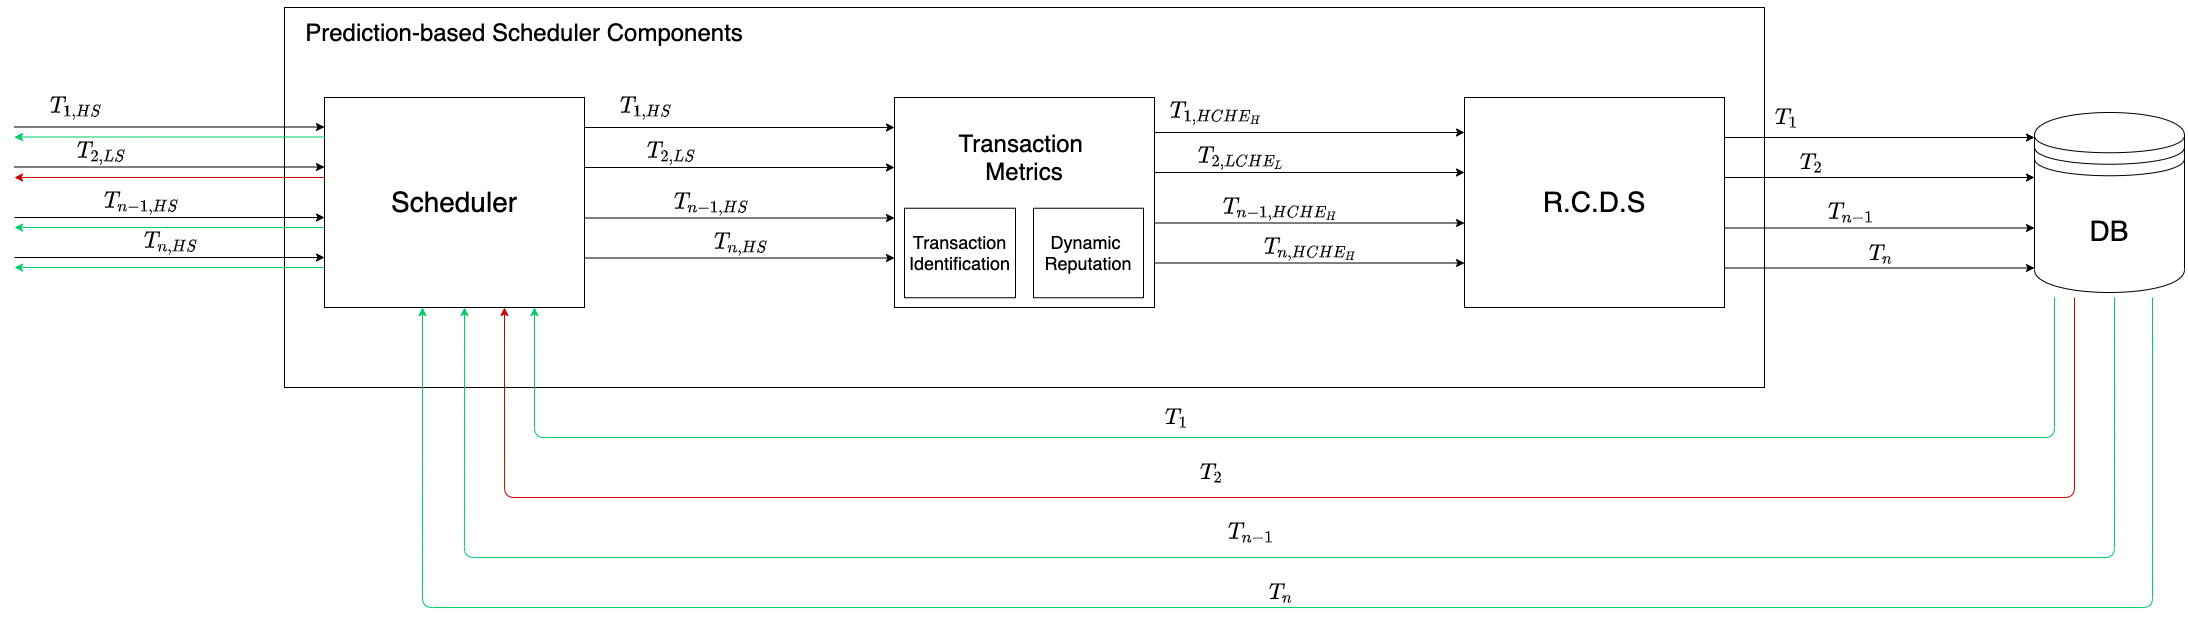
\includegraphics[width=\textwidth]{images/SystemModel_Overall}
\caption{Overall System Model of Prediction-based Scheduler}
\label{fig:system_model_overall}
\end{figure}

\subsection{Dynamic Reputation for Transactions}
In the previous section, the categorization of the transaction is assumed in order to continue forward with the decision model. This section of the dissertation involves the work needed to establish a dynamic reputation management system to allow for dynamic reputation. It involves building a reputation score for each transaction based on the transactions ranking of efficiency, commits, system aborts, and user aborts. Once a reputation score is provided we can then use dynamic reputation management to dynamically promote and demote transactions. This then allows the system to adapt to its environment dynamically. The work discussed in this area is documented in Chapter \ref{chap:dynamic_reputation}.

% Figure \ref{fig:system_model_overall} displays the system model for the work done for transactional correctness and building a dynamic reputation for transactions.
\section{Dissertation Outline}
The rest of this dissertation is organized as follows: Chapter \ref{chap:prediction_based_scheduler} outlines the research done in regards to transactional correctness while preserving concurrent operations within a web service environment. This work is published in \cite{ravan_ensuring_2020}. Chapter \ref{chap:dynamic_reputation} addresses the research done in order to build a reputation for a given transaction that is dynamic to its environment and its changing attributes. This work is submitted to ACM Transactions on Information Systems and awaiting response. Chapter \ref{chap:outline} contains the outline of the dissertation. Chapter \ref{chap:future_work} addresses the future work needed to adapt the prediction-based scheduler in Chapter \ref{chap:prediction_based_scheduler} and Chapter \ref{chap:dynamic_reputation} to a multi-level secure database and other possible solutions. Chapter \ref{chap:conclusion} contains the concluding remarks regarding all areas of research.
